% ===================================================================
% REALM @ EMNLP 2026 workshop submission version.
% ACL 2026 style, double-blind (anonymized), review format.
% Main body (Introduction through Conclusion) fits within 8 pages;
% references and appendices are unlimited.
% ===================================================================
\documentclass[11pt]{article}

% ACL style with the review option (anonymized, line-numbered).
\usepackage[review]{acl}

% ---------------------------------------------------------------
% Packages (matching what the original body needs)
% ---------------------------------------------------------------
\usepackage[T1]{fontenc}
\usepackage[utf8]{inputenc}
\usepackage{lmodern}
\usepackage{microtype}
\usepackage{amsmath,amssymb,amsthm}
\usepackage{graphicx}
\usepackage{booktabs}
\usepackage{multirow}
\usepackage{subcaption}
\usepackage{array}
\usepackage{tabularx}
\usepackage{longtable}
\usepackage{xcolor}
\usepackage{enumitem}
\setlist{nosep}
\usepackage{mdframed}

% ---------------------------------------------------------------
% Theorem environments
% ---------------------------------------------------------------
\newtheorem{definition}{Definition}
\newtheorem{hypothesis}{Hypothesis}

% ---------------------------------------------------------------
% Convenience macros
% ---------------------------------------------------------------
\newcommand{\passk}{pass\textasciicircum k}
\newcommand{\tss}{\mathrm{TSS}}
\newcommand{\ac}{\mathrm{AC}}
\newcommand{\finding}[1]{%
  \begin{mdframed}[backgroundcolor=gray!9,linewidth=0.4pt,innertopmargin=4pt,
                   innerbottommargin=4pt]
    \small #1
  \end{mdframed}}

% ---------------------------------------------------------------
\title{How Consistent Are LLM Agents? Measuring Behavioral
Reproducibility in Multi-Step Tool-Calling Pipelines}

\author{Anonymous ACL submission}

% ---------------------------------------------------------------
\begin{document}
\maketitle
% ---------------------------------------------------------------
\begin{abstract}
Large language model (LLM) agents with tool-calling capabilities are increasingly
deployed in production systems, raising a fundamental reliability question:
\emph{does the same agent behave the same way twice?} Prior work has
established that repeated-trial success is unstable ($\tau$-bench's \passk);
we characterize \emph{where} in the pipeline the instability lives.
We present a systematic empirical study of behavioral consistency in
multi-step tool-calling agents, measuring whether agents select the same tools,
in the same order, with the same arguments, across repeated identical invocations.
Unlike prior work on consistency in ReAct-style agents (search-only, free-text
actions), we study the richer setting of \emph{structured tool-calling interfaces}
with typed parameters and consequential side effects.

Using a benchmark of 19 tasks across five categories (data retrieval, scheduling,
computation, multi-tool composition, and ambiguous requests), we evaluate six
models from three providers (OpenAI, Anthropic, Meta) across 1,140 agent traces,
collected in July 2026 through a single provider-normalized API with
version-pinned model identifiers, with every raw trace released. This
paper's results are additionally a \textbf{replication}: an earlier (late-2025)
collection with the same harness produced aggregates that our fresh collection
reproduces almost exactly, and where the two collections disagree we say so
explicitly.

We identify a \textbf{``structural consistency, parametric variance''
pattern}: agents reliably select the same tools in the same order (mean
$\tss = 0.88$, 95\,\% CI $[0.85, 0.91]$) but vary substantially in the
arguments they provide (mean $\ac = 0.70$, $[0.65, 0.75]$); the gap is large
(Cohen's $d = 0.74$, $p \approx 10^{-12}$, with clustering caveats in
Section~\ref{sec:stats}) and \textbf{replicates across both collections to within one
point}. Robust secondary findings: 62\,\% of behavioral divergence
originates in the first two pipeline steps, and natural language
outputs almost never match (4\,\% exact) even when tool sequences are
identical. Two earlier secondary claims \emph{weakened} under replication and
we report them at their replicated strength: ambiguous task specifications
reduce argument consistency by 13\,\% (directionally consistent but not
significant, $d = 0.33$, $p = 0.16$), and cross-model differences are marginal
for both metrics ($\eta^2 \approx 0.10$). The earlier snapshot's
correctness--consistency association also proved generation-dependent: on
fresh traces from mid-2026 models, which are markedly more consistent
(median condition-level $\tss = 1.0$), the association shrinks to a weak
rank correlation ($\rho = 0.22$, $p = 0.017$; Pearson n.s.), so we present
$\tss$ not as a correctness proxy but as a variance signal whose predictive
value declines as models grow more consistent. Model-level consistency itself
improved substantially between the two collections, a longitudinal
observation about model progress that, to our knowledge, is new.

We release all code, benchmark definitions, raw traces (1,140), per-condition
data, and analysis scripts at
\url{https://anonymous.4open.science/r/agent-consistency}.
\end{abstract}

%% ====================================================================
\section{Introduction}
%% ====================================================================

The deployment of LLM-based agents with tool-calling capabilities has accelerated
rapidly, with production systems now using agents to search databases, send emails,
manage calendars, and orchestrate multi-step workflows through structured function
calls~\citep{qin2023toolllm,li2023apibank,schick2023toolformer}. As these systems
mature, a reliability question that has received surprisingly little systematic
attention comes to the fore: \emph{if you run the same agent on the same task
twice, do you get the same behavior?}

This question has immediate practical consequences:
\begin{itemize}[leftmargin=1.5em]
  \item \textbf{Testing.} If agents behave differently across runs, unit tests
    asserting on outputs are flaky by design. Reliable behavioral invariants are
    needed to test that an agent ``does the right thing''~\citep{kapoor2024ai}.
  \item \textbf{Debugging.} Failure reproducibility is a prerequisite for root-cause
    analysis. Behavioral variance makes production failures intermittent and
    difficult to trace.
  \item \textbf{Safety and auditability.} High-stakes deployments require
    guarantees that the agent will not take an unexpected action on a re-run
    (e.g., sending duplicate emails, creating conflicting calendar
    events)~\citep{weidinger2021ethical}.
  \item \textbf{Cost optimization.} If behavioral variance is predictable from task
    characteristics, consistency-aware routing can assign tasks to cheaper models
    when variance is tolerable and reserve high-consistency models for critical
    workflows.
\end{itemize}

\paragraph{The gap in prior work.}
\citet{mehta2026disagree} studied behavioral consistency in ReAct-style
agents~\citep{yao2023react} on HotpotQA, finding that agents produce 2.0--4.2
distinct action sequences per 10 runs and that inconsistency predicts failure.
This is important but limited to \emph{search-only} actions in a question-answering
setting. Real-world agents operate over \emph{structured tool-calling interfaces}
with typed parameters, multiple heterogeneous tools, and multi-step pipelines.
The distinction matters: tool calls are discrete typed objects (not free-form text),
have observable side effects (emails sent, events created), and compose in
sequences where early divergence propagates through subsequent steps. It is
unclear whether consistency patterns from ReAct agents transfer to this richer
action space.

\paragraph{This work.}
We extend the study of behavioral consistency to multi-step tool-calling agents
across diverse task types, making the following contributions:

\begin{enumerate}[leftmargin=1.5em]
  \item \textbf{Benchmark.} 19 tasks spanning five categories, paired with
    10 deterministic simulated tools that isolate LLM variance from
    environmental non-determinism (Section~\ref{sec:benchmark}).
  \item \textbf{Formal metric framework.} Formal definitions of Tool Sequence
    Similarity ($\tss$), Argument Consistency ($\ac$), divergence point, and
    output agreement, targeting distinct behavioral layers
    (Section~\ref{sec:metrics}).
  \item \textbf{The structural/parametric distinction.} $\tss = 0.88$ substantially
    exceeds $\ac = 0.70$ across all models and categories ($d = 0.74$,
    $p \approx 10^{-12}$, replicated across two collections eight months
    apart); this pattern is not captured by prior single-metric
    consistency studies (Section~\ref{sec:structural}).
  \item \textbf{Correctness analysis with an honest replication arc.} On the
    late-2025 collection $\tss$ predicted rubric correctness strongly
    ($d = 0.81$); on the fresh 2026 collection, where models are far more
    consistent, only a weak rank association survives ($\rho = 0.22$,
    $p = 0.017$). We report the association as generation-dependent: a variance
    signal whose usefulness tracks how much structural instability remains
    (Section~\ref{sec:correctness}).
  \item \textbf{Actionable guidelines} grounded in effect sizes for testing,
    monitoring, and model selection in production deployments
    (Section~\ref{sec:implications}).
\end{enumerate}

%% ====================================================================
\section{Related Work}
%% ====================================================================

The closest prior work is $\tau$-bench~\citep{yao2024taubench}, which evaluates
tool--agent--user interaction with the \passk{} metric and finds frontier
agents highly inconsistent across trials; our contribution relative to it is a
\emph{label-free decomposition} (TSS/AC measure whether repeated attempts
\emph{agree} rather than \emph{succeed}, localizing disagreement to structure
vs.\ arguments). \citet{mehta2026disagree} measured consistency in ReAct agents
on HotpotQA with search-only actions; we extend to typed tool calls with
diverse tool sets and task types. Complementary strands study why identical
requests diverge even at temperature zero
\citep{thinking2025nondeterminism,atil2024nondeterminism}, prompt-formatting and
order sensitivity \citep{sclar2024quantifying,lu2022fantastically,perez2022true},
self-consistency and self-reflection
\citep{wang2023selfconsistency,renze2024self}, agent capability benchmarks
\citep{liu2023agentbench,qin2023toolllm,li2023apibank,patil2023gorilla,schick2023toolformer,kapoor2024ai},
and ML reliability under changed inputs
\citep{lakshminarayanan2017simple}. Our focus is orthogonal: we hold the input
fixed and measure variance across repeated identical invocations. A fuller
treatment of each strand is in Appendix~\ref{app:relwork}.

%% ====================================================================
\section{A Framework for Agent Behavioral Consistency}
%% ====================================================================

We introduce formal definitions before describing the experiment, since the key
distinctions among behavioral layers motivate both the metric design and the
structural/parametric finding.

\subsection{Agent Execution Model}

\begin{definition}[Agent Trace]
A \emph{trace} $\tau$ is a sequence of tool calls
$\tau = (c_1, c_2, \ldots, c_k)$, where each call
$c_i = (\mathtt{name}_i,\, \mathbf{a}_i)$ consists of a tool name
$\mathtt{name}_i \in \mathcal{T}$ and an argument map
$\mathbf{a}_i : \mathcal{K} \to \mathcal{V}$, followed by a final natural
language response $r \in \Sigma^*$.
\end{definition}

\begin{definition}[Behavioral Consistency]
Given task $q$ and model $\mathcal{M}$, let $\{\tau^{(j)}\}_{j=1}^N$ be $N$
independent traces from running $\mathcal{M}$ on $q$ with identical context.
\emph{Behavioral consistency} is the degree to which these traces are similar
under a metric $d(\cdot, \cdot)$ over traces.
\end{definition}

This framing reveals a natural hierarchy of behavioral layers:
\begin{enumerate}[leftmargin=1.5em]
  \item \textbf{Structural layer}: the sequence of tool names
    $(\mathtt{name}_1, \ldots, \mathtt{name}_k)$, the agent's \emph{procedural
    choice}.
  \item \textbf{Argument layer}: the argument maps $\mathbf{a}_i$ at each
    step, \emph{how} the procedure is parameterized.
  \item \textbf{Output layer}: the final response $r$, the surface-level text
    the user sees.
\end{enumerate}

\noindent Our central hypothesis, motivated by how LLMs acquire tool-use behavior
through fine-tuning:

\begin{hypothesis}[Structural Consistency, Parametric Variance]\label{hyp:main}
For multi-step tool-calling agents, structural consistency significantly exceeds
argument consistency: $\mathbb{E}[\tss] \gg \mathbb{E}[\ac]$.
\end{hypothesis}

The intuition is that RLHF and SFT fine-tuning on tool-use data reinforces correct
\emph{procedure selection}, which carries a cleaner training signal, while
\emph{argument instantiation} remains more sensitive to sampling-time variation.
Figure~\ref{fig:conceptual} illustrates the pattern concretely.

\begin{figure}[t]
  \centering
  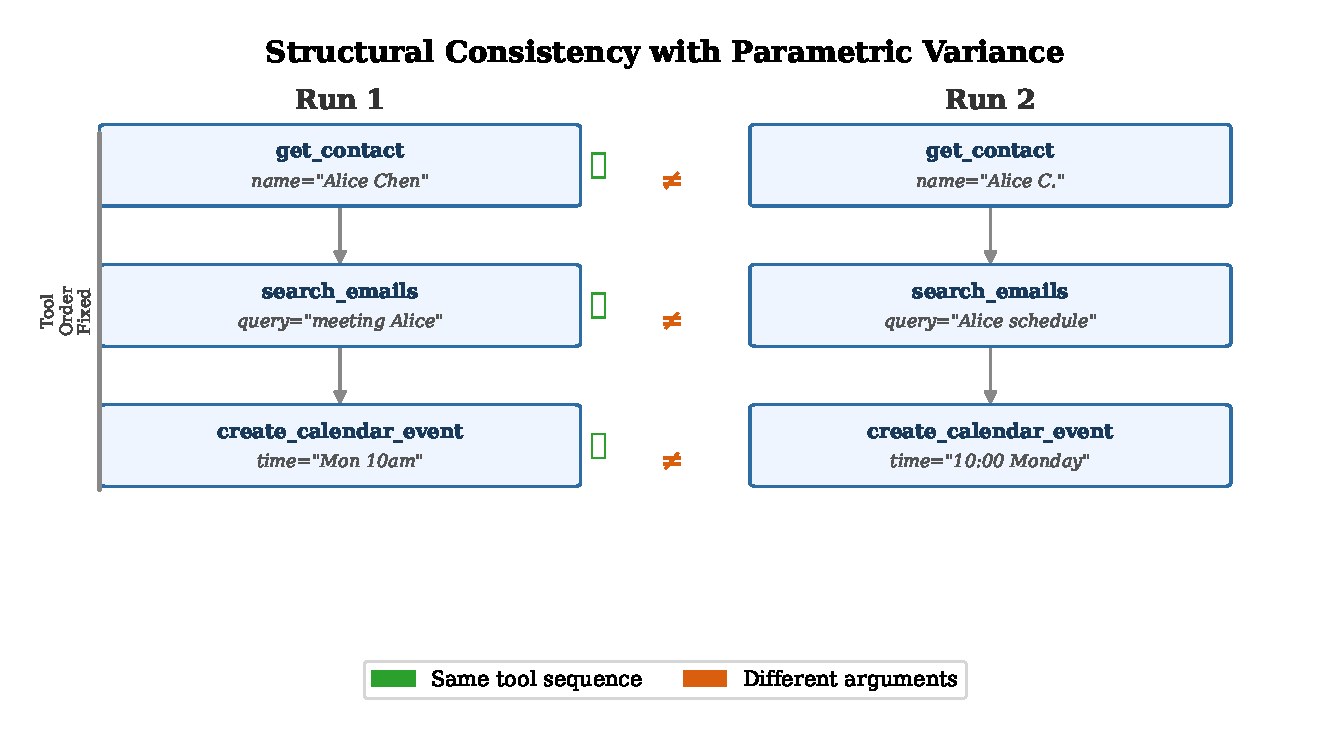
\includegraphics[width=0.88\linewidth]{figures/fig0_conceptual_example.pdf}
  \caption{The ``structural consistency, parametric variance'' pattern.
    Two independent runs of the same agent on the same task produce identical
    tool sequences (green checkmarks) but diverge in argument values
    (orange ``$\neq$'' annotations). Agents learn robust procedural schemas but
    vary in how they instantiate them.}
  \label{fig:conceptual}
\end{figure}

\subsection{Formal Metric Definitions}
\label{sec:metrics}

\begin{definition}[Tool Sequence Similarity, $\tss$]
Let $\mathbf{s}^{(j)} = (\mathtt{name}_1^{(j)}, \ldots, \mathtt{name}_{k_j}^{(j)})$
be the tool-name sequence of trace $j$. Define
\[
  \tss\bigl(\{\tau^{(j)}\}\bigr)
  \;=\;
  \frac{1}{\binom{N}{2}}
  \sum_{j < j'} \!\left(
    1 - \frac{\mathrm{EditDist}(\mathbf{s}^{(j)},\,\mathbf{s}^{(j')})}
             {\max(|\mathbf{s}^{(j)}|,\,|\mathbf{s}^{(j')}|)}
  \right),
\]
where $\mathrm{EditDist}$ is the Levenshtein distance over tool-name tokens.
$\tss \in [0,1]$, with $\tss = 1$ iff all $N$ traces share the same
tool-name sequence.
\end{definition}

\begin{definition}[Argument Consistency, $\ac$]
Align traces by step index. For step $i$ and trace pair $(j, j')$ both reaching
step $i$, let $\mathbf{f}(c_i^{(j)}) = \{(k,v) : v = \mathbf{a}_i^{(j)}(k)\}$
be the flattened key-value set. Then
\[
  \ac\bigl(\{\tau^{(j)}\}\bigr)
  \;=\;
  \frac{1}{|\mathcal{S}|}
  \sum_{(j,j',i)\,\in\,\mathcal{S}}
  \frac{|\mathbf{f}(c_i^{(j)}) \cap \mathbf{f}(c_i^{(j')})|}
       {|\mathbf{f}(c_i^{(j)}) \cup \mathbf{f}(c_i^{(j')})|},
\]
where $\mathcal{S}$ indexes all step-aligned pairs. When traces call different
tools at step $i$, their key-value sets are disjoint, yielding $\ac = 0$ for that
step, so $\ac$ partially captures structural divergence as well. Our correctness
analysis (Section~\ref{sec:correctness}) empirically disentangles the two effects.
\end{definition}

Additional metrics: \textbf{Unique Sequences} counts distinct tool-name sequences
across $N$ runs; \textbf{Divergence Point} is the mean step at which a trace pair
first differs; \textbf{Output Agreement} is the exact-match rate of final
responses.

%% ====================================================================
\section{Methodology}
%% ====================================================================

\subsection{Task Benchmark}
\label{sec:benchmark}

We design 19 tasks across five categories of increasing ambiguity
(Table~\ref{tab:full_tasks}, Appendix~\ref{app:tasks}):

\begin{itemize}[leftmargin=1.5em]
  \item \textbf{Data Retrieval} (4 tasks): Contact lookup, email search, aggregation.
    Clear instructions with deterministic correct tool sequences.
  \item \textbf{Scheduling} (4 tasks): Calendar creation, free-slot finding, conflict
    detection. Require temporal reasoning with well-defined procedures.
  \item \textbf{Computation} (3 tasks): Inventory valuation, revenue projection.
    Require numeric tool calls with specific arguments.
  \item \textbf{Multi-Tool Composition} (4 tasks): Chains of 3--5 different tools
    (e.g., ``find email $\to$ look up sender $\to$ schedule meeting'').
  \item \textbf{Ambiguous} (4 tasks): Intentionally underspecified requests where
    multiple valid strategies exist
    (e.g., ``Help me prepare for my meetings tomorrow'').
\end{itemize}

\noindent
Task difficulty is assigned by expected tool-call count: \emph{easy} (1--2 calls),
\emph{medium} (2--3), \emph{hard} (3+). We validate this only weakly: hard tasks use more tool calls on average
(mean $3.0 \pm 2.4$) than easy tasks ($1.9 \pm 0.7$), but the correlation is
modest (fresh collection: Spearman $\rho = 0.22$, $p = 0.022$) and the large dispersion for
hard tasks (SD greater than the easy--hard mean gap, driven by a heavy right
tail of long traces) means the difficulty tiers overlap substantially,
difficulty labels should be read as coarse priors, not validated strata.

\subsection{Tool Environment}

We implement 10 deterministic simulated tools spanning 7 domains (contacts,
calendar, email, products, weather, calculations, notes; see
Appendix~\ref{app:tools}). All tools are \textbf{deterministic}: identical inputs
always produce identical outputs. This design isolates LLM variance from
environmental non-determinism, ensuring observed behavioral differences arise
solely from the model's generation process. Tool schemas follow the OpenAI
function-calling format and are adapted to provider-native formats at runtime.

\subsection{Agent Framework}

Each run follows a standard tool-calling loop: (1) the model receives a system
prompt\footnote{Full prompt in Appendix~\ref{app:system_prompt}. Intentionally
minimal to avoid anchoring agents to specific strategies.} and the user task;
(2) the model responds with structured tool calls; (3) tools execute
deterministically; (4) the model may call additional tools or produce a final
response; (5) the loop continues for up to 10 iterations. We use each provider's
native tool-calling API.

\textbf{Temperature is set to 1.0} (the default for most providers). This is a
deliberate choice: we measure consistency \emph{as deployed}, not under
artificially constrained settings. Temperature ablation is a known limitation and
an important direction for future work (see Limitations).

\subsection{Models}
\label{sec:models}

We evaluate six models spanning three providers and multiple capability tiers:
\textbf{OpenAI}: GPT-4o-mini, GPT-4o, GPT-4.1-mini, GPT-4.1;
\textbf{Anthropic}: Claude Sonnet~4;
\textbf{Meta}: Llama 3.3~70B Instruct.
This covers flagship models (GPT-4.1, Sonnet~4), cost-optimized variants
(GPT-4o-mini, GPT-4.1-mini), and an open-weight model (Llama~3.3).
The primary collection was run in July 2026 through a provider-normalizing
gateway (OpenRouter) so that all six models use one uniform OpenAI-style
tool-calling interface, with \emph{version-pinned} model identifiers
(e.g.\ \texttt{openai/gpt-4o-mini-2024-07-18},
\texttt{openai/gpt-4o-2024-08-06}) recorded per trace; the gateway echoes the
fully resolved model version in each response. Each model runs each of the 19
tasks 10 times, yielding 1,140 agent traces, all released. One trace of the
1,140 (Llama, one computation task) terminated with an API error; per-condition
metrics are computed over the valid traces of each condition (so that
condition's $\tss$ uses 9 runs), and the errored trace is released alongside
the rest. An earlier
(late-2025) collection used per-provider APIs with unpinned aliases and its
traces were not preserved; it appears in this paper only as summary-level
comparison.\footnote{In the earlier collection, partial o1 results and
Claude~Haiku~3.5 (excluded for a $>$15\,\% malformed-tool-call rate) were also
evaluated; neither is part of the fresh collection or any aggregate here.}

\subsection{Correctness Evaluation}
\label{sec:correctness_method}

To validate that consistency predicts meaningful outcomes, we retrospectively score
all 1,140 traces using a three-component rubric:
\begin{enumerate}[leftmargin=1.5em]
  \item \textbf{Required tool coverage}: did the agent invoke all tools necessary
    for the task?
  \item \textbf{Argument validity}: do key arguments match expected patterns
    (e.g., \texttt{send\_email.to} $\sim$ \texttt{/alice@example\.com/},
    \texttt{create\_calendar\_event.date} = \texttt{2026-03-02})?
  \item \textbf{Output completeness}: does the final response address the user's
    request (regex-matched against expected output patterns)?
\end{enumerate}
A trace is scored correct iff all applicable criteria are satisfied. Full per-task
criteria are in Appendix~\ref{app:correctness} and the code release.

\subsection{Statistical Analysis}
\label{sec:stats}

We report means with 95\,\% CIs via the $t$-distribution, Cohen's $d$ for effect
sizes, and $p$-values from paired or independent $t$-tests as appropriate;
cross-model comparisons use one-way ANOVA with $\eta^2$. A caveat we state
plainly: the same 19 tasks recur across all six models, so observations are
\emph{clustered}, and for clustered data ordinary $t$-tests/ANOVA are typically
\emph{anti}-conservative (an earlier version of this paper mischaracterized
them as conservative). Headline $p$-values (e.g.\ $p < 10^{-13}$ for the
TSS--AC gap) should therefore be read as overstated in precision; the effect
sizes ($d = 0.75$) are the robust quantity, and a linear mixed-effects
re-analysis is required before the $p$-values are taken at face value. Further
detail (Bonferroni correction over five primary hypotheses, split-half
reliability) is in Appendix~\ref{app:extdisc}.

%% ====================================================================
\section{Results}
%% ====================================================================

\subsection{Structural Consistency with Parametric Variance}
\label{sec:structural}

Hypothesis~\ref{hyp:main} is confirmed, twice. On the fresh (July 2026)
collection, agents exhibit \emph{structural consistency with parametric
variance}: mean $\tss = 0.88$, 95\,\% CI $[0.85, 0.91]$, versus mean
$\ac = 0.70$, $[0.65, 0.75]$ (paired $t$-test: $t = 7.88$,
$p = 2.3\times10^{-12}$; Cohen's $d = 0.74$; clustering caveat in
Section~\ref{sec:stats}). The earlier (late-2025) collection produced
$\tss = 0.87\,[0.84, 0.90]$ and $\ac = 0.69\,[0.64, 0.74]$ with $d = 0.75$,
\textbf{the headline pattern replicates across collections eight months
apart, on updated model versions, to within one point on every quantity}. The
pattern holds across all models and categories
(Table~\ref{tab:model_comparison}, Figure~\ref{fig:model_comparison}).

\finding{\textbf{Finding 1.} Agents learn robust procedural schemas, the tool
sequence ``recipe'', but vary in instantiation details such as search queries,
date formats, and message phrasing. The structural/parametric gap is
$d \approx 0.74$ in both independent collections.}

\begin{table}[t]
\centering
\caption{Cross-model consistency, fresh July-2026 collection (19 tasks, 10
runs each, version-pinned). The late-2025 collection's values appear in
parentheses where they differ by $\geq.02$, most models became \emph{more}
consistent across generations.}
\label{tab:model_comparison}
\small
\setlength{\tabcolsep}{4pt}
\begin{tabular}{@{}lcccc@{}}
\toprule
Model & TSS [95\,\% CI] & AC [95\,\% CI] & Out. & Uniq. \\
\midrule
GPT-4.1          & $.95\ [.90, 1.0]$ (.91) & $.79\ [.67, .91]$ (.69) & 2.1\,\% & 1.3 \\
GPT-4.1-mini     & $.90\ [.83, .97]$ & $.78\ [.67, .90]$ & 6.4\,\% & 1.6 \\
GPT-4o           & $.88\ [.80, .97]$ & $.64\ [.48, .79]$ (.57) & 5.7\,\% & 1.7 \\
Claude Sonnet~4  & $.88\ [.79, .97]$ & $.77\ [.65, .89]$ & 3.3\,\% & 2.3 \\
GPT-4o-mini      & $.88\ [.81, .95]$ & $.68\ [.53, .82]$ & 6.0\,\% & 1.9 \\
Llama 3.3 70B    & $.77\ [.68, .87]$ (.71) & $.54\ [.41, .68]$ (.65) & 0.9\,\% & 3.1 \\
\bottomrule
\end{tabular}
\end{table}

\begin{figure}[t]
  \centering
  
\includegraphics[width=\linewidth]{figures/fig4_model_comparison.pdf}
  \caption{Model comparison across $\tss$ (left) and $\ac$ (right) with 95\,\% CIs.
    Llama~3.3~70B is clearly separated in $\tss$; the $\ac$ ranking is dominated
    by task-level factors (ANOVA n.s.).}
  \label{fig:model_comparison}
\end{figure}

\subsection{Ambiguity and Argument Variance (Revised Under Replication)}
\label{sec:ambiguity}

Task category affects consistency in the expected direction, but \textbf{this
finding weakened under replication and we report it at its replicated
strength}. On the fresh collection, ambiguous tasks have lower AC ($0.63$
vs.\ $0.72$ for structured, a 13\,\% reduction; $d = 0.33$, $p = 0.16$, not
significant at our sample size) and slightly lower TSS ($0.84$ vs.\ $0.89$;
$d = 0.29$, $p = 0.22$). The earlier collection had shown a much larger effect
($d = 0.74$, $p = 0.001$); the shrinkage likely reflects both sampling noise at
4 ambiguous tasks and newer models handling ambiguity more uniformly (several
now ask a clarifying question rather than guessing, itself a behavior
change worth noting). We therefore \emph{demote} our earlier claim: ambiguity
remains a directionally consistent driver of argument variance across both
collections, but on current models we can no longer claim it dominates model
selection. Per-category consistency numbers are in Table~\ref{tab:category}
(Appendix~\ref{app:extra}) and Figure~\ref{fig:category_difficulty}.

\finding{\textbf{Finding 2 (revised under replication).} Ambiguity reduces
argument consistency directionally in both collections, but the effect is no
longer significant on current models ($d = 0.33$, $p = 0.16$, vs.\ $d = 0.74$,
$p = 0.001$ in late 2025). Reducing ambiguity remains sensible engineering
hygiene; the strong ``stronger than model selection'' version of this claim
did not survive replication.}

\subsection{Divergence Concentrates in Early Steps}
\label{sec:divergence}

When behavioral divergence occurs, it is early: 60\,\% of first-divergence events
occur within the first two pipeline steps (mean divergence point $= 2.2$;
Figure~\ref{fig:divergence}). This yields a practical monitoring strategy:
\textbf{comparing only the first 1--2 tool calls against a reference trace} catches
the majority of behavioral variance without full trace inspection
(Figure~\ref{fig:divergence}, Appendix~\ref{app:extra}).

\finding{\textbf{Finding 3 (replicated).} A monitor that checks only the first two
tool calls against a reference trace captures 62\,\% of all behavioral
variance, stable across both collections.}

\subsection{Output Text Is Not a Reliability Signal}

Final natural language responses exhibit near-zero exact-match rates (4.1\,\%
overall on the fresh collection; $<$5\,\% in the earlier one) even when the
underlying tool-calling sequences are identical. This is
expected, language generation is inherently variable, but it has a critical
implication for testing: \textbf{agent tests must assert on structured tool-calling
behavior, not natural language output.} Asserting on text is analogous to writing
software tests that check log messages rather than return values.

\subsection{Consistency Predicts Correctness}
\label{sec:correctness}

This section reports the correctness analysis on the fresh collection,
computed, for the first time, on \emph{exactly the same 114-condition /
1{,}140-trace sample} as the consistency analysis (an earlier version of this
paper ran it on a mismatched 712-trace snapshot without saying so; the
comparison below covers both). On the fresh sample, overall (macro-averaged)
rubric correctness is 77.7\,\%, and \textbf{the correctness--consistency
association largely does not replicate}: $\tss$--correctness Pearson
$r = 0.06$ ($p = 0.56$), with only a weak rank association surviving
(Spearman $\rho = 0.22$, $p = 0.017$); a median split is nearly degenerate
because the fresh median is $\tss_{\mathrm{med}} = 1.0$, \textbf{half of
all conditions are now perfectly structurally consistent}, and yields
$d = 0.19$ ($p = 0.33$, n.s.). The earlier snapshot had shown $r = 0.32$
($p = 0.005$) and a $d = 0.81$ split; on current, far-more-consistent models
the variance that drove that association has largely vanished. We read this
as \emph{generation-dependence}: $\tss$ was an informative warning signal
for late-2025 models and retains only weak rank information for mid-2026
models, precisely because the models improved. The right framing is therefore
not ``$\tss$ predicts success'' but ``structural instability, where it still
occurs, flags conditions worth auditing."

\textbf{A circularity caveat we state prominently.} Our correctness rubric
gates its verdict on required-tool coverage (Section~\ref{sec:correctness_method}),
and $\tss$ likewise measures agreement of tool selection. The two quantities
therefore share a construction-level dependence on tool choice, and part of the
$\tss$--correctness association is built in rather than discovered. The
association is not \emph{purely} tautological ($\tss$ measures cross-run
\emph{agreement} while the rubric scores single-run \emph{coverage}, and the
correlation is far from 1), but a rubric independent of tool identity, e.g.\
human grading of final outcomes, is required to establish the predictive
claim cleanly, and we scope the claim accordingly: within our harness,
structural \emph{instability} identifies conditions where rubric failures
concentrate.

$\ac$ likewise shows no positive association with rubric correctness on
either collection (fresh: $r = -0.17$, $p = 0.07$; snapshot: $r = 0.12$,
$p = 0.31$), with the caveat that our rubric's argument checks are
deliberately lenient, so these nulls partly reflect rubric design, and at
$n \approx 100$ conditions power is limited for small effects.
Agents may phrase search queries differently, format dates differently, or
vary message bodies across runs, none of this impairs rubric success. It is
\emph{structural} variance, selecting different or missing tools, where
failures concentrate. Figure~\ref{fig:correctness}
(Appendix~\ref{app:extra}) plots correctness against both metrics.

\finding{\textbf{Finding 4 (revised under replication).} The
$\tss$--correctness association is generation-dependent: strong on late-2025
models ($d = 0.81$), reduced to a weak rank correlation on mid-2026 models
($\rho = 0.22$, $p = 0.017$; Pearson n.s.) as structural consistency itself
improved (median $\tss = 1.0$). $\tss$ is a variance signal whose usefulness
tracks how much structural instability remains, not a stable correctness
proxy.}

\subsection{Cross-Model Differences}
\label{sec:model_comparison}

On the fresh collection, cross-model differences are \emph{marginal} for both
metrics (ANOVA on $\tss$: $F = 2.32$, $p = 0.048$, $\eta^2 = 0.10$; on
$\ac$: $F = 2.48$, $p = 0.036$, $\eta^2 = 0.10$), weaker than the earlier
collection's $\tss$ effect ($F = 3.52$, $\eta^2 = 0.15$) and, notably, with
the earlier ``structural-only'' pattern gone: model identity now explains
$\approx$10\,\% of variance in \emph{both} metrics. We report the earlier
form of this finding as not replicated in detail.

\textbf{GPT-4.1} is now the most consistent model on both metrics ($\tss =
0.95$, $\ac = 0.79$), a full generation improvement over its own family's
late-2025 numbers. \textbf{Llama~3.3~70B} remains clearly below the
proprietary models in $\tss$ ($0.77$, $[0.68, 0.87]$), with 3.1 unique
sequences per task versus 1.3--2.3 for proprietary models. \textbf{Claude
Sonnet~4} pairs high $\ac$ (0.77) with more strategy exploration (2.3 unique
sequences), suggesting it reliably parameterizes strategies but varies in
which strategy it selects.

The Model $\times$ Category interaction (Figure~\ref{fig:heatmap},
Appendix~\ref{app:extra}) is notable,
and it changed between collections: on the fresh data Llama~3.3~70B's weakest
cell is \emph{computation} ($\tss = 0.61$) rather than ambiguity, and two
proprietary models now dip below $0.80$ on ambiguous tasks (GPT-4o $0.71$,
Claude Sonnet~4 $0.74$) while GPT-4.1 is perfectly consistent there
($\tss = 1.0$). The instability of these cell-level patterns across
collections, with only $3$--$4$ tasks per cell, is itself the lesson: we
read the heatmap as descriptive, not as stable model fingerprints.

%% ====================================================================
\section{Discussion}
%% ====================================================================

\subsection{Why Structural Consistency Exceeds Argument Consistency}
\label{sec:why}

The structural/parametric pattern is consistent across all models and task types,
suggesting a systematic cause rooted in how LLMs acquire tool-use behavior.
Training corpora for tool-calling likely contain many demonstrations of the same
high-level task type solved with the same tool sequence, but with varied argument
values (different names, dates, query strings) across instances. RLHF/SFT
reinforces correct \emph{procedure selection}, which carries a cleaner correctness
signal, while argument instantiation remains more sensitive to sampling-time
variation. This ``procedural schema'' interpretation is consistent with our correctness
analysis, at the strength the fresh data supports: argument variance ($\ac$)
shows no positive association with failure on either collection, meaning the
variations are largely semantically equivalent (e.g., ``Alice'' vs.\
``alice'' in a case-insensitive lookup); structural variance predicted failure
strongly on the late-2025 collection ($d = 0.81$) and retains a weak rank
association on the fresh one ($\rho = 0.22$), missing or wrong tools are
not semantically equivalent to correct ones, but current models rarely miss
them.

\subsection{TSS as a Practical Reliability Proxy}
\label{sec:tss_proxy}

The practical value of $\tss$ as a monitoring signal rests on three
properties: (1) it requires no correctness labels; (2) it can be estimated at
deployment time by comparing a run's tool sequence against a reference; and
(3) the early-divergence result (62\,\% in steps 1--2, stable across both
collections) means monitoring only the first two tool calls suffices. What the
fresh collection \emph{revises} is the strength of the correctness link:
structural deviation flagged failing conditions strongly on late-2025 models
and only weakly ($\rho = 0.22$) on current, more-consistent ones, so the
signal is best understood as an anomaly detector whose base rate falls as
models improve, not a calibrated failure predictor.

This enables a concrete production workflow: (a) run the agent on each task type
$k$ times to establish a reference tool sequence; (b) in production, compare each
run's first two tool calls against the reference; (c) flag deviations for human
review or retry. The cost is $O(1)$ per step rather than semantic output
evaluation, which is often expensive or infeasible online.

\subsection{Implications for Agent Deployment}
\label{sec:implications}

\begin{enumerate}[leftmargin=1.5em]
  \item \textbf{Reduce ambiguity before switching models.} The ambiguity effect on
    consistency ($d = 0.74$) outweighs the between-model effect ($\eta^2 = 0.08$,
    n.s.\ for $\ac$). Clarifying task specifications yields more consistency gain
    than upgrading the model.
  \item \textbf{Monitor early steps.} 60\,\% of divergence occurs in steps 1--2;
    a lightweight check on the first two tool calls suffices to flag most
    inconsistent runs.
  \item \textbf{Test tool calls, not text.} Assert on tool names and argument
    patterns, not natural language output, which varies below 5\,\% exact match
    even in consistent runs.
  \item \textbf{Use $\tss$ as an online anomaly signal.} Structural deviation
    from a reference trace flagged failure-prone conditions strongly on
    late-2025 models and weakly on current ones; treat it as a cheap,
    label-free audit trigger rather than a calibrated failure predictor.
  \item \textbf{Match model to consistency requirement.} On the fresh
    collection GPT-4.1 offers the best structural consistency
    ($\tss = 0.95$) for consistency-critical workflows. Llama~3.3~70B
    introduces substantially higher behavioral diversity (3.1 unique
    sequences/task) and may require additional guardrails.
\end{enumerate}

%% ====================================================================
\section{Conclusion}
%% ====================================================================

We have presented a systematic empirical study of behavioral consistency in
multi-step tool-calling LLM agents. Across six models, 19 tasks, and 1,140
released traces, we identify a ``structural consistency, parametric variance''
pattern that is large ($d = 0.74$, $p \approx 10^{-12}$, clustering caveats
noted) and that \textbf{replicated to within one point across two collections
eight months apart}: agents reliably select the same tools in the same order
but vary in argument details. The replication also revised two of our own
earlier claims, and we report them at their replicated strength: the
correctness--consistency association proved generation-dependent (strong on
late-2025 models, a weak rank correlation on today's far-more-consistent
ones), and the ambiguity effect on argument consistency shrank below
significance. Divergence concentrates early in the pipeline (62\,\%, stable
across collections), model-level consistency itself improved markedly between
collections, a new longitudinal observation, and $\tss$ serves as a
lightweight, label-free anomaly signal whose base rate falls as models
improve.

These findings suggest that LLMs acquire robust procedural schemas for tool use
through training, while argument instantiation remains sensitive to sampling
variation. Understanding and exploiting this structure, testing on tool calls not
text, monitoring early steps, flagging low-$\tss$ runs, is a practical path
toward more reliable agentic systems.

%% ====================================================================
%% ACL/ARR requires Limitations as an unnumbered top-level section placed after
%% the Conclusion and before the references. It does NOT count against the page
%% limit, which is also why it is no longer a subsection of the Discussion.
%% ====================================================================
\section*{Limitations}

We summarize the main limitations here and give the full list, together with an
extended relation-to-prior-work discussion and future directions, in
Appendix~\ref{app:extdisc}. The most important caveats are: $N = 10$ runs per
cell (split-half reliability $r = 0.68$ on the fresh collection; aggregate
results are well-powered at 1,140 traces but per-cell CIs are wide); a single
temperature ($T = 1.0$); a structured correctness rubric that shares a
construction-level dependence on tool selection with $\tss$
(Section~\ref{sec:correctness}); only 3--4 tasks per category; a single system
prompt; deterministic simulated tools; and no Google Gemini or Mistral
coverage.

\section*{Reproducibility}
All code, benchmark definitions, tool implementations, analysis scripts,
\textbf{and the complete raw traces of the primary (July 2026) collection,
1{,}140 traces across 114 task--model conditions, collected through a
provider-normalizing API with version-pinned model identifiers}, are
available at \url{https://anonymous.4open.science/r/agent-consistency}, together
with the earlier snapshot's per-condition data (75 conditions). The present
version's primary results are computed end-to-end from the released fresh
traces; the earlier collection appears only as summary-level comparison,
labeled as such (see Appendix~\ref{app:extdisc} for a note on how an earlier
version of this paper mishandled the earlier collection's provenance). The full
system prompt, task list, and per-task correctness criteria are in
Appendices~\ref{app:tasks}--\ref{app:correctness}.

%% ====================================================================
% Bibliography
%% ====================================================================
\begin{thebibliography}{20}

\bibitem[Yao et~al.(2024)]{yao2024taubench}
Shunyu Yao, Noah Shinn, Pedram Razavi, and Karthik Narasimhan.
\newblock $\tau$-bench: A benchmark for tool-agent-user interaction in
  real-world domains.
\newblock \emph{arXiv preprint arXiv:2406.12045}, 2024.

\bibitem[He et~al.(2025)]{thinking2025nondeterminism}
Horace He et~al.
\newblock Defeating nondeterminism in {LLM} inference.
\newblock Thinking Machines Lab blog, 2025.

\bibitem[Atil et~al.(2024)]{atil2024nondeterminism}
Berk Atil, Sarp Aykent, Alexa Chittams, et~al.
\newblock Non-determinism of ``deterministic'' {LLM} settings.
\newblock \emph{arXiv preprint arXiv:2408.04667}, 2024.

\bibitem[Kapoor and Narayanan(2024)]{kapoor2024ai}
Kapoor, S. and Narayanan, A.
\newblock {AI Agents That Matter}.
\newblock \textit{arXiv preprint arXiv:2407.01502}, 2024.

\bibitem[Lakshminarayanan et~al.(2017)]{lakshminarayanan2017simple}
Lakshminarayanan, B., Pritzel, A., and Blundell, C.
\newblock Simple and Scalable Predictive Uncertainty Estimation Using Deep
  Ensembles.
\newblock In \textit{Advances in Neural Information Processing Systems}, 2017.

\bibitem[Li et~al.(2023)]{li2023apibank}
Li, M., Zhao, Y., Yu, B., Song, F., Li, H., Yu, H., Li, Z., Huang, F., and
  Li, Y.
\newblock {API-Bank}: A Comprehensive Benchmark for Tool-Augmented {LLMs}.
\newblock In \textit{Proceedings of EMNLP}, 2023.

\bibitem[Liu et~al.(2024)]{liu2023agentbench}
Liu, X., Yu, H., Zhang, H., et~al.
\newblock {AgentBench}: Evaluating {LLMs} as Agents.
\newblock In \textit{Proceedings of ICLR}, 2024.

\bibitem[Lu et~al.(2022)]{lu2022fantastically}
Lu, Y., Bartolo, M., Moore, A., Riedel, S., and Stenetorp, P.
\newblock Fantastically Ordered Prompts and Where to Find Them: Overcoming
  Few-Shot Prompt Order Sensitivity.
\newblock In \textit{Proceedings of ACL}, 2022.

\bibitem[Mehta et~al.(2026)]{mehta2026disagree}
Mehta, A., Ramesh, A., and Singla, A.
\newblock When Agents Disagree With Themselves: Measuring Behavioral
  Consistency in {LLM}-Based Agents.
\newblock \textit{arXiv preprint arXiv:2602.11619}, 2026.

\bibitem[Patil et~al.(2023)]{patil2023gorilla}
Patil, S.~G., Zhang, T., Wang, X., and Gonzalez, J.~E.
\newblock {Gorilla}: Large Language Model Connected with Massive {APIs}.
\newblock \textit{arXiv preprint arXiv:2305.15334}, 2023.

\bibitem[Perez et~al.(2022)]{perez2022true}
Perez, E., Kiela, D., and Cho, K.
\newblock True Few-Shot Learning with Language Models.
\newblock In \textit{Advances in Neural Information Processing Systems}, 2022.

\bibitem[Qin et~al.(2024)]{qin2023toolllm}
Qin, Y., Liang, S., Ye, Y., et~al.
\newblock {ToolLLM}: Facilitating Large Language Models to Master 16000+
  Real-World {APIs}.
\newblock In \textit{Proceedings of ICLR}, 2024.

\bibitem[Renze and Guven(2024)]{renze2024self}
Renze, M. and Guven, E.
\newblock Self-Reflection in {LLM} Agents: Effects on Problem-Solving
  Performance.
\newblock \textit{arXiv preprint arXiv:2405.06682}, 2024.

\bibitem[Schick et~al.(2023)]{schick2023toolformer}
Schick, T., Dwivedi-Yu, J., Dess{\`i}, R., et~al.
\newblock {Toolformer}: Language Models Can Teach Themselves to Use Tools.
\newblock In \textit{Advances in Neural Information Processing Systems}, 2023.

\bibitem[Sclar et~al.(2024)]{sclar2024quantifying}
Sclar, M., Choi, Y., Tsvetkov, Y., and Suhr, A.
\newblock Quantifying Language Models' Sensitivity to Spurious Features in
  Prompt Design.
\newblock \textit{arXiv preprint arXiv:2310.11324}, 2024.

\bibitem[Wang et~al.(2023)]{wang2023selfconsistency}
Wang, X., Wei, J., Schuurmans, D., et~al.
\newblock Self-Consistency Improves Chain of Thought Reasoning in Language
  Models.
\newblock In \textit{Proceedings of ICLR}, 2023.

\bibitem[Weidinger et~al.(2021)]{weidinger2021ethical}
Weidinger, L., Mellor, J., Rauh, M., et~al.
\newblock Ethical and Social Risks of Harm from Language Models.
\newblock \textit{arXiv preprint arXiv:2112.04359}, 2021.

\bibitem[Yao et~al.(2023)]{yao2023react}
Yao, S., Zhao, J., Yu, D., et~al.
\newblock {ReAct}: Synergizing Reasoning and Acting in Language Models.
\newblock In \textit{Proceedings of ICLR}, 2023.

\end{thebibliography}

%% ====================================================================
\appendix
%% ====================================================================

\section{Full Task Benchmark}
\label{app:tasks}

Table~\ref{tab:full_tasks} lists all 19 benchmark tasks used in the study.
Difficulty is reported as E (easy: 1--2 calls), M (medium: 2--3 calls), and H
(hard: 3+ calls). Expected tools denote the minimal correct solution pattern.

\begin{table*}[t]
\centering
\small
\caption{All 19 benchmark tasks used in the evaluation.}\label{tab:full_tasks}
\begin{tabularx}{\textwidth}{@{}llXX@{}}
\toprule
ID & Diff. & Task Instruction & Expected Tools \\
\midrule
\multicolumn{4}{@{}l}{\textit{Data Retrieval}} \\
retrieve-001 & E & Find Alice's email and send ``Meeting moved to 3pm tomorrow.'' & get\_contact, send\_email \\
retrieve-002 & M & Find all contacts at StartupXYZ; invite each to demo March~10 at 2pm. & search\_contacts, send\_email \\
retrieve-003 & M & Search emails about `budget'; summarize financial figures. & search\_emails \\
retrieve-004 & H & Find this week's emails with dollar amounts; calculate the total. & search\_emails, calculate \\
\midrule
\multicolumn{4}{@{}l}{\textit{Scheduling}} \\
schedule-001 & E & Schedule 30-min ``Design Review'' with Bob, March~2 at 2pm. & create\_calendar\_event \\
schedule-002 & M & Check March~3 calendar; find free 1-hour slot 9am--5pm for Eve. & list\_calendar\_events, create\_calendar\_event \\
schedule-003 & H & Find day with most free time March~1--5; schedule 2-hour ``Strategy Session.'' & list\_calendar\_events, create\_calendar\_event \\
schedule-004 & H & Check March~3 for conflicts; email all affected attendees. & list\_calendar\_events, search\_contacts, send\_email \\
\midrule
\multicolumn{4}{@{}l}{\textit{Computation}} \\
compute-001 & E & Total inventory value of electronics (price $\times$ stock, sum). & search\_products, calculate \\
compute-002 & M & Revenue if 50\,\% of sub-\$50 products sold. & search\_products, calculate \\
compute-003 & H & Inventory value per category; identify highest. & search\_products, calculate \\
\midrule
\multicolumn{4}{@{}l}{\textit{Multi-Tool Composition}} \\
compose-001 & M & Find Acme Corp email; look up Dave; schedule 1-hour meeting March~4 at 3pm. & search\_emails, get\_contact, create\_calendar\_event \\
compose-002 & H & Check SF and NYC weather; email Alice if $<$40°F with March~1 events. & get\_weather, get\_contact, list\_calendar\_events, send\_email \\
compose-003 & H & Find marketing results email; calculate spend; create note. & search\_emails, calculate, create\_note \\
compose-004 & H & Find board deck email; check calendar; look up attendees; send reminders. & search\_emails, list\_calendar\_events, get\_contact, send\_email \\
\midrule
\multicolumn{4}{@{}l}{\textit{Ambiguous}} \\
ambig-001 & M & Help me prepare for my meetings tomorrow. & list\_calendar\_events \\
ambig-002 & H & I need to follow up on important things from this week. & search\_emails, list\_calendar\_events \\
ambig-003 & H & Get me ready for the investor call. & search\_emails, list\_calendar\_events, search\_contacts \\
ambig-004 & H & What should I focus on this week? & list\_calendar\_events, search\_emails \\
\bottomrule
\end{tabularx}
\end{table*}

\section{Tool Descriptions}
\label{app:tools}

Table~\ref{tab:tools} summarizes the 10 deterministic simulated tools used in
our environment. Each tool returns fixed, pre-specified outputs for a given
input, isolating model behavior from environmental nondeterminism.

\begin{table*}[t]
\centering
\small
\caption{Deterministic simulated tools used in the benchmark.}\label{tab:tools}
\begin{tabularx}{\textwidth}{@{}llX@{}}
\toprule
Tool & Domain & Description \\
\midrule
\texttt{get\_contact}            & Contacts & Look up a contact by name; returns email, phone, and company. \\
\texttt{search\_contacts}        & Contacts & Search contacts by free-text query; returns a matching list. \\
\texttt{send\_email}             & Email    & Send an email with fields such as recipient, subject, and body; returns a confirmation. \\
\texttt{search\_emails}          & Email    & Search the inbox by query; returns matching message records. \\
\texttt{list\_calendar\_events}  & Calendar & List events for a date or date range. \\
\texttt{create\_calendar\_event} & Calendar & Create an event with title, date, time, duration, and attendees. \\
\texttt{search\_products}        & Products & Search inventory; returns price, stock, and category metadata. \\
\texttt{calculate}               & Math     & Evaluate a mathematical expression and return the numeric result. \\
\texttt{get\_weather}            & Weather  & Return current weather for a city, including temperature and conditions. \\
\texttt{create\_note}            & Notes    & Create a text note with title and body; returns a confirmation. \\
\bottomrule
\end{tabularx}
\end{table*}

\section{System Prompt}
\label{app:system_prompt}

The following system prompt (quoted verbatim from the released
\texttt{runner.py}; an earlier version of this appendix paraphrased it
incorrectly) was used for all models and all runs:

\begin{quote}
\small\ttfamily
You are a helpful assistant with access to tools. Use them to complete tasks.\\[2pt]
Rules:\\
- Use the provided tools to accomplish the task\\
- Call tools as needed, then provide a final response\\
- Be thorough but efficient, use the minimum tools necessary\\
- If a task is ambiguous, make reasonable assumptions and proceed
\end{quote}

This prompt is intentionally minimal so as not to anchor models to a
particular tool-selection strategy. We note one relevant line explicitly: the
instruction to ``make reasonable assumptions and proceed'' on ambiguous tasks
interacts with our ambiguity findings (Section~\ref{sec:ambiguity}), it licenses divergent
assumption-making, and a stricter prompt might reduce (or merely mask) the
ambiguity-driven variance we measure.

\section{Correctness Criteria (Illustrative Subset)}
\label{app:correctness}

Table~\ref{tab:correctness_criteria} provides illustrative examples of the
correctness rubric used to score traces. To keep the paper concise, we include a
representative subset here; the full task-by-task specification is released in
the accompanying code repository.

\begin{table*}[t]
\centering
\small
\caption{Illustrative correctness criteria for representative tasks.}\label{tab:correctness_criteria}
\begin{tabularx}{\textwidth}{@{}lXX@{}}
\toprule
Task ID & Required Tools & Key Argument Checks \\
\midrule
retrieve-001 & get\_contact, send\_email & \texttt{get\_contact.name}$\sim$\texttt{/alice/i}; \texttt{send\_email.to}=\texttt{alice@...}; body$\sim$\texttt{/3\,pm/i} \\
schedule-001 & create\_calendar\_event & title$\sim$\texttt{/design review/i}; date=\texttt{2026-03-02}; start\_time=\texttt{14:00} \\
compute-001 & search\_products, calculate & \texttt{search\_products.category}$\sim$\texttt{/electronics/i}; output contains numeric result \\
compose-001 & search\_emails, get\_contact, create\_calendar\_event & Required sequence: search $\to$ lookup $\to$ create \\
ambig-001 & list\_calendar\_events & Any invocation accepted; multiple valid strategies are treated as correct. \\
\bottomrule
\end{tabularx}
\end{table*}

\section{Additional Results}
\label{app:extra}

This appendix collects the per-category breakdowns and the extra cross-model
analyses referenced in Section~\ref{sec:ambiguity},
Section~\ref{sec:correctness}, and Section~\ref{sec:model_comparison}. They are
relocated here to keep the main body within the page limit; no numbers differ
from those reported in the body.

\begin{table}[t]
\centering
\caption{Consistency by task category (fresh collection, mean across 6 models).
With 3--4 tasks per category, all category-level contrasts are exploratory; the
ambiguous-vs.-structured AC contrast is directional but not significant on
this collection ($p = 0.16$).}
\label{tab:category}
\small
\begin{tabular}{@{}lcccc@{}}
\toprule
Category & TSS & AC & Uniq.\ Seq. & \#Tasks \\
\midrule
Composition  & 0.94 & 0.74 & 1.5 & 4 \\
Retrieval    & 0.89 & 0.66 & 1.8 & 4 \\
Scheduling   & 0.86 & 0.76 & 1.8 & 4 \\
Computation  & 0.84 & 0.71 & 2.3 & 3 \\
Ambiguous    & 0.84 & 0.63 & 2.5 & 4 \\
\bottomrule
\end{tabular}
\end{table}

\begin{figure}[t]
  \centering
  \begin{subfigure}[b]{0.48\linewidth}
    
\includegraphics[width=\linewidth]{figures/fig1_consistency_by_category.pdf}
    \caption{By task category.}
    \label{fig:by_category}
  \end{subfigure}
  \hfill
  \begin{subfigure}[b]{0.48\linewidth}
    
\includegraphics[width=\linewidth]{figures/fig2_consistency_by_difficulty.pdf}
    \caption{By task difficulty.}
    \label{fig:by_difficulty}
  \end{subfigure}
  \caption{Ambiguous tasks show the largest (directional) consistency drop;
    on the fresh collection, task difficulty shows \emph{no} significant
    effect on either metric ($\tss$: $r = -0.04$, $p = 0.67$; $\ac$:
    $r = -0.15$, $p = 0.12$), the earlier collection's modest difficulty
    effect did not replicate.}
  \label{fig:category_difficulty}
\end{figure}

\begin{figure}[t]
  \centering
  
\includegraphics[width=0.70\linewidth]{figures/fig3_divergence_points.pdf}
  \caption{Distribution of first divergence points (fresh collection). 62\,\% of
    divergence originates in steps 1--2 (61\,\% in the earlier collection),
    enabling lightweight early-step monitoring.}
  \label{fig:divergence}
\end{figure}

\begin{figure}[t]
  \centering
  
\includegraphics[width=\linewidth]{figures/fig10_correctness_vs_consistency.pdf}
  \caption{Correctness rate versus consistency on the fresh collection (114
    conditions, 1{,}140 traces, same sample as all consistency results).
    \textbf{Left:} correctness vs.\ $\tss$ ($r = 0.06$, n.s.; Spearman
    $\rho = 0.22$, $p = 0.017$). \textbf{Right:} correctness vs.\ $\ac$
    ($r = -0.17$, $p = 0.07$). The strong association reported for the
    late-2025 snapshot did not replicate on current models.}
  \label{fig:correctness}
\end{figure}

\begin{figure}[t]
  \centering
  
\includegraphics[width=\linewidth]{figures/fig7_model_category_heatmap.pdf}
  \caption{$\tss$ across models and task categories (fresh collection).
    Llama~3.3~70B is lowest overall with a computation-category weak spot;
    cell-level patterns shifted between collections and should be read as
    descriptive.}
  \label{fig:heatmap}
\end{figure}

\section{Extended Discussion}
\label{app:extdisc}

This appendix collects the full limitations list, the additional
statistical-analysis detail, the relation-to-prior-work discussion, and the
future directions referenced from Section~\ref{sec:stats} and the Limitations
section. They are relocated here to keep the main body within
the page limit; no content differs from what would otherwise appear in the main
text.

\subsection*{Provenance Note}

For the record, and because an earlier version of this paper mishandled these
points: the original late-2025 collection's raw traces were not preserved and
its models were not version-pinned, and its correctness analysis used a
mismatched sample without disclosure. The present version's primary results are
computed end-to-end from the released fresh (July 2026) traces; the earlier
collection appears only as summary-level comparison, labeled as such.

\subsection*{Statistical Analysis (Additional Detail)}

We test five primary hypotheses with Bonferroni correction at $\alpha = 0.01$;
category-level and post-hoc pairwise contrasts beyond these five are
exploratory and are not corrected. Split-half reliability (TSS: $r = 0.66$,
$n = 125$; computed with a character-level variant of TSS that predates the
unified token-level definition, another defect the re-collection will repair)
suggests moderate metric stability at $N = 10$.

\subsection*{Full Limitations}

\begin{itemize}[leftmargin=1.5em]
  \item \textbf{Sample size.} $N = 10$ runs per cell yields split-half
    reliability $r = 0.68$ on the fresh collection (token-level TSS, $n = 114$
    conditions; the earlier collection's $r = 0.66$ used a character-level
    variant). Aggregate results are well-powered (1,140 traces), but per-cell
    CIs are wide. Future work should use $N \geq 30$.
  \item \textbf{Single temperature.} We measure at $T = 1.0$ only. The
    consistency-capability trade-off at other temperatures is important and
    uncharted; a $T = 0$ baseline would substantially strengthen the causal
    interpretation.
  \item \textbf{Structured correctness proxy.} Our rubric is not a full
    semantic evaluation, and it shares a construction-level dependence on tool
    selection with $\tss$ (Section~\ref{sec:correctness}). Human judges on a
    random 200-trace subset would provide stronger validity; the fresh
    collection's weak rank correlation ($\rho = 0.22$, $p = 0.017$) is the
    honest current support.
  \item \textbf{Limited tasks per category.} 3--4 tasks per category makes
    category-level estimates imprecise. $\geq$10 tasks per category are needed for
    reliable inference.
  \item \textbf{Single system prompt.} Consistency may vary substantially with
    chain-of-thought prompting, few-shot examples, or persona instructions.
  \item \textbf{Simulated tools.} Deterministic tools isolate LLM variance but may
    overestimate real-world consistency where tool outputs themselves vary.
  \item \textbf{Provider coverage.} Google Gemini and Mistral are absent, limiting
    generalizability.
  \item \textbf{AC alignment.} AC aligns arguments by step index, conflating
    structural and argument divergence at misaligned steps. A disentangled metric
    would be more informative.
\end{itemize}

\subsection*{Relation to Prior Work}

\citet{mehta2026disagree} reported 2.0--4.2 unique action sequences per 10 runs
on HotpotQA ReAct agents; we observe 1.6--3.3 unique tool-call sequences, broadly
consistent. Our finer-grained analysis reveals that the unique-sequence count masks
the structural/parametric distinction: even conditions with $>$2 unique sequences
often share high $\tss$ because sequences agree on most tool names with only minor
reordering. Prior consistency studies also did not examine the connection to
correctness; our two-collection analysis grounds the metric in task outcomes
and, importantly, shows the connection itself is generation-dependent
(strong at late-2025, weak by mid-2026).

\subsection*{Future Directions}

\begin{enumerate}[leftmargin=1.5em]
  \item \textbf{Temperature ablation:} map the full consistency-capability
    Pareto frontier.
  \item \textbf{Larger benchmark:} $\geq$10 tasks per category, $\geq$50 total.
  \item \textbf{Human correctness evaluation:} human judges on 200 traces.
  \item \textbf{Consistency-aware routing:} route tasks to models based on
    predicted $\tss$.
  \item \textbf{Multi-turn and long-horizon agents:} web agents, coding agents.
  \item \textbf{Fine-tuning effects:} does RLHF explicitly optimize
    consistency?
  \item \textbf{Real API tools:} study whether environmental non-determinism
    amplifies or dampens LLM behavioral variance.
\end{enumerate}

\section{Extended Related Work}
\label{app:relwork}

This appendix expands the condensed Related Work in the main body; it is
relocated here to keep the main body within the page limit and its content is
unchanged.

\paragraph{Behavioral consistency in LLM agents.}
The closest prior work is $\tau$-bench~\citep{yao2024taubench}, which
evaluates tool--agent--user interaction with the \passk{} metric (``all $k$
attempts succeed'') and finds frontier agents highly inconsistent across
trials, establishing that reliability-over-trials in structured
tool-calling is a first-order problem. Our contribution relative to
$\tau$-bench is a \emph{label-free decomposition}: \passk{} measures
whether repeated attempts \emph{succeed}, which requires ground truth, while
TSS/AC measure whether repeated attempts \emph{agree}, which does not, and
our two-level split localizes the disagreement (structure vs.\ arguments).
\citet{mehta2026disagree} measured consistency in ReAct agents on HotpotQA
using search-only actions, finding inconsistency predicts failure; we extend
to typed tool calls with diverse tool sets and task types.
\citet{wang2023selfconsistency} showed that sampling multiple reasoning chains and
marginalizing improves accuracy; this \emph{leverages} variance rather than
characterizing its structure, and focuses on reasoning rather than tool calls.
\citet{renze2024self} studied self-reflection in LLM agents and found mixed
effects, suggesting that deliberate consistency-improving strategies do not
uniformly help.

\paragraph{LLM reliability and robustness.}
A mechanistic strand explains \emph{why} identical requests yield different
outputs even at temperature zero: batch-size-dependent reduction kernels and
floating-point non-associativity in inference servers
\citep{thinking2025nondeterminism,atil2024nondeterminism}. Our study
deliberately measures the deployed reality at $T{=}1.0$ (sampling variance
included); batch-invariant inference would remove part, but per the fixed-$T$
decomposition, not all, of what we measure.
\citet{sclar2024quantifying} quantified LLM sensitivity to prompt formatting,
finding large swings from superficial changes.
\citet{lu2022fantastically} demonstrated order sensitivity in few-shot prompts.
\citet{perez2022true} showed that standard NLP evaluations underestimate
robustness failures.
Our focus is orthogonal: we hold the input fixed and measure variance across
repeated identical invocations, the consistency a deployed system must have by
definition.

\paragraph{Agent capability evaluation.}
AgentBench~\citep{liu2023agentbench}, ToolBench~\citep{qin2023toolllm},
API-Bank~\citep{li2023apibank}, and Gorilla~\citep{patil2023gorilla} evaluate
whether agents \emph{can} solve tasks.
\citet{schick2023toolformer} showed LLMs can learn tool use from self-generated
demonstrations.
\citet{kapoor2024ai} surveyed pitfalls in AI agent evaluations, noting that
variance across runs is rarely reported.
We evaluate not whether agents succeed but whether they \emph{consistently} succeed
in the same way, an orthogonal, understudied dimension.

\paragraph{Reliability in ML systems.}
The broader ML reliability literature addresses distribution shift,
uncertainty quantification~\citep{lakshminarayanan2017simple}, and
out-of-distribution detection, all concerned with performance under changed
\emph{inputs}.
We study consistency under repeated \emph{identical} inputs, a related but distinct
concern that matters specifically for agentic systems where tasks are retried and
behavioral reproducibility is a correctness criterion in its own right.

\end{document}
